
% TODO: Change the tone of the introduction, talk about exploring the
% TODO: proposed changes

\section{Experiment Design}
\label{sec:experiment}

In this paper we propose three improvements for the GAModel algorithm
that generates earthquake risk models using GA: A reduced
representation that limits the search space of the algorithm, a hybrid
model generation that uses domain knowledge, and the pre-processing of
the data using Spectral Clustering.

We are interested in determine what effect these improvements have on
the generation of earthquake risk models. To achieve this, we execute
a series of simulation experiments. In these experiments, we generate
earthquake models for each combination of the above modifications,
using historical earthquake catalog data from the Japanese
arquipelago.

We compare these simulations through the accuracy of the resulting
models, represented by the log-likelihood between the model and the
catalog data.

\subsection{Experiment Design}

%% TODO: Problem -- comparison is incomplete: Spectral clustering is not
%% tested on Tohoku and Kansai. How to write it?

We compare four 

% - Goals/List of experiments
%% - Analysis of parameters (Clustering/Others)
%% - Comparison of the influence of the modifications

% - How we execute the experiments
%% - For each of the proposed analysis, we run
%% the evolutionary algorithm to generate a 
%% risk model, and we compare the resulting models

% - How we analyze the experiments
%% Comparison is done as...


\subsubsection*{Claus' Extracts}

Statistical analysis: ANOVA on the populational means

Tukey HSD for significant differences on ANOVA

- 

\subsubsection*{Old Text}

The first experiment was made to compare the all the models proposed
with each other and to discover which method would achieve higher
log-likelihood values. We created some scenarios (space/time regions),
and we applied the methods for for the regions of Kanto, Kansai,
Touhoku and East Japan for a given year (2005-2010) with earthquakes
with depth lesser than 100km. We also used 3 kinds of catalogues with
the minimum magnitude of 3.0: the JMA and the declustered catalogues
form the Window method and the SLC method.

We compared the means of the models log-likelihood values using the
ANOVA test. If a group of variables considered for the ANOVA test
showed no statistically significant difference, we applied the Paired
Student t-test, in the case all groups showed statistically
significant difference, the Tukey HSD methodology analysis was used.



%%%%%%%%%%%%%%%%%%%%%%%%%%%%%%%%%%%%%%%%%%%%%%%%%%%%%%%%%%%%%%%%%%%%%%%5
\subsection{Data Sets}

%%% Four Regions (Kansai, Touhoku, EastJapan, Kanto)
%%% Six time periods (2005,2006,2007,2008,2009,2010)
%%% Depth cut-offs: 100
%%% Magnitude cutoff: 3


The earthquake catalog from the Japanese arquipelago were obtained
from the \emph{Japan Meteorological Agency} (JMA) webpage.

% - How we obtained the data sets

% - Explanation of the data sets (locations)

% - Parameters of the data sets


The goal of this research is to find existing patterns in the
occurrence of earthquakes. For that it is essential to access trustful
data and to explore its details. From the {\it Japan Meteorological
  Agency} web page we obtained earthquake data about earthquakes in
Japan. In this data there are information about earthquakes that
happened in or nearby Japan, with the variables: time of the
occurrence, magnitude, latitude and longitude and epicentre depth, for
the years of 2000 to 2013.

During the preprocessing phase, we discovered a higher number of
occurrences of earthquakes during the year of 2011, when a 9.0 $M_w$
earthquake happened, see Section~\ref{chapter1}. This earthquake
triggered too many after called aftershocks in all Japan. It is
considered that big earthquakes may cause others
earthquakes~\cite{zhuang2004analyzing}. In~Figure \ref{ocorrenciasAno}
it is possible to visualise a great number of earthquakes for the year
of 2011. Because of this abnormal behaviour and because we decided to
focus on more stable occurrences, we limited the training base to
earthquakes until 2010.

\begin{figure}[]
\centering
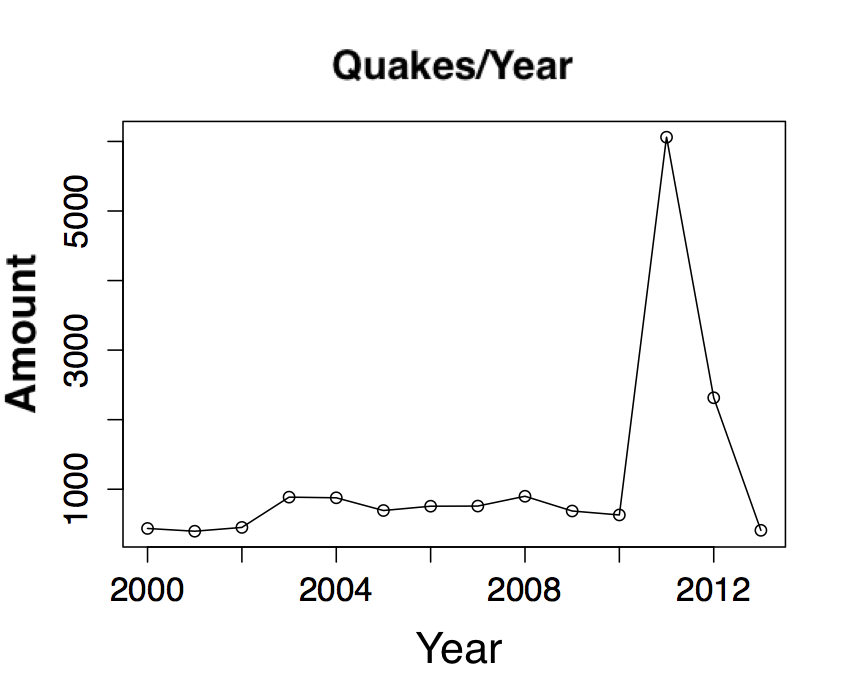
\includegraphics[scale=0.5]{img/ocorrenciasAno.png}
\caption{Amount of earthquake by year.}
\label{ocorrenciasAno}
\end{figure}


Based on the statement done before and considering that we want
earthquakes that follow more stable patterns, we selected the ones
that happened in land areas or very shallow sea areas, with maximum
depth of 100km.

For the experiments, the data was changed into slices for every
year. Each slice is as follows: if the base contains data about a time
interval of 10 years, it will be split in 10 slices.

We also selected some sub-areas in Japan to better extract and
understand earthquakes characteristics and patterns. Those areas are
Kanto, Kansai, Touhoku and East Japan. The Figure~\ref{alljapan} shows
how we defined them.

\begin{figure}
	\centering
	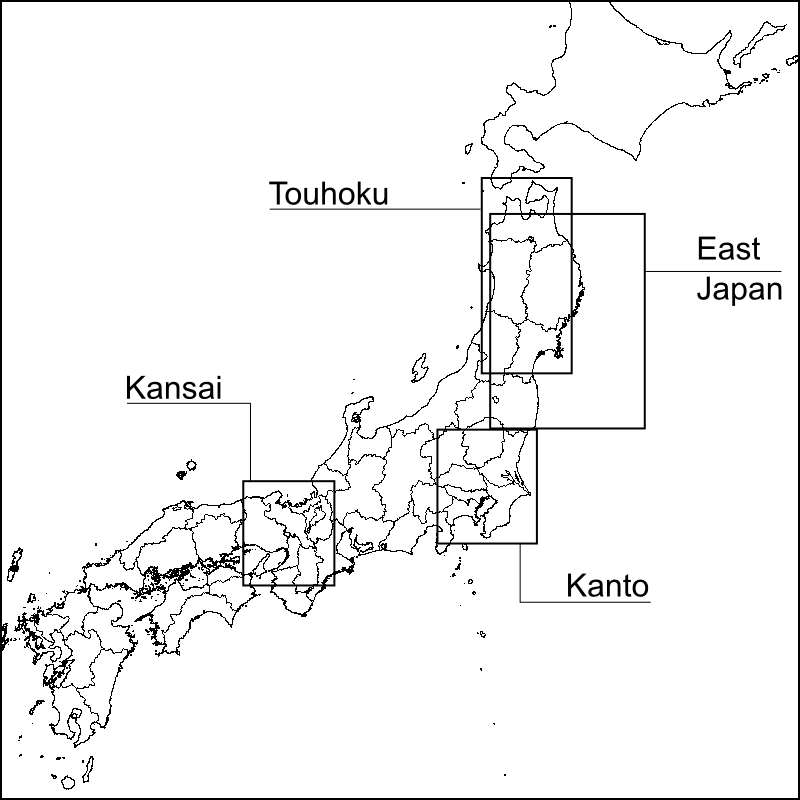
\includegraphics[scale=0.25]{img/alljapan.png}
	\caption{Japan and the areas used in this studied.}
	\label{alljapan}
\end{figure}


The regions are described as follows:

\textbf{Kanto} Kanto is the region around Tokyo. It is an area with
high seismologic activity during the years we studied. Its coordinates
are 34.8 North, 138.8 West, with 2025 bins. Each bin covers an area of
approximately 25km$^2$.

\textbf{Kansai} Kansai is the region that includes Kyoto, Osaka and
many others historical cities. In this area, rather than Kanto area,
there is a small seismic activity. Its coordinates are 34 North, 134.5
West, with 1600 bins. Each bin covers an area of approximately
25km$^2$.

\textbf{Touhoku} Touhoku is the region in the North of the main
Japanese island. It has some clusters of seismic activities during the
years we studied. Its coordinates are 37.8 North, 139.8 West, with 800
bins. Each bin covers an area of approximately 100km$^2$.

\textbf{East Japan} Is the region that is related with the east coast
of Japan. It is the most different area, because it has earthquakes
that happened both in land or in the sea. It was in this region that
the 9.0 $M_w$ earthquake happened. Its coordinates are 37 North, 140
West, with 1600 bins. Each bin covers an area of approximately
100km$^2$.

\subsubsection{Depth Histogram of Earthquakes}


The patterns of earthquakes are dependent of the epicentre. We wanted
to explore the relation between the depth of the earthquakes and how
would our models behave on those situations.

In Figure~\ref{histogramQuakes}, it is possible to understand that
most of the earthquakes happened with depths smaller or equal to 100
km. The earthquakes deeper than 100 km are fewer and more distant, as
it is in the same Figure.\\

\begin{figure}[]
	\centering
	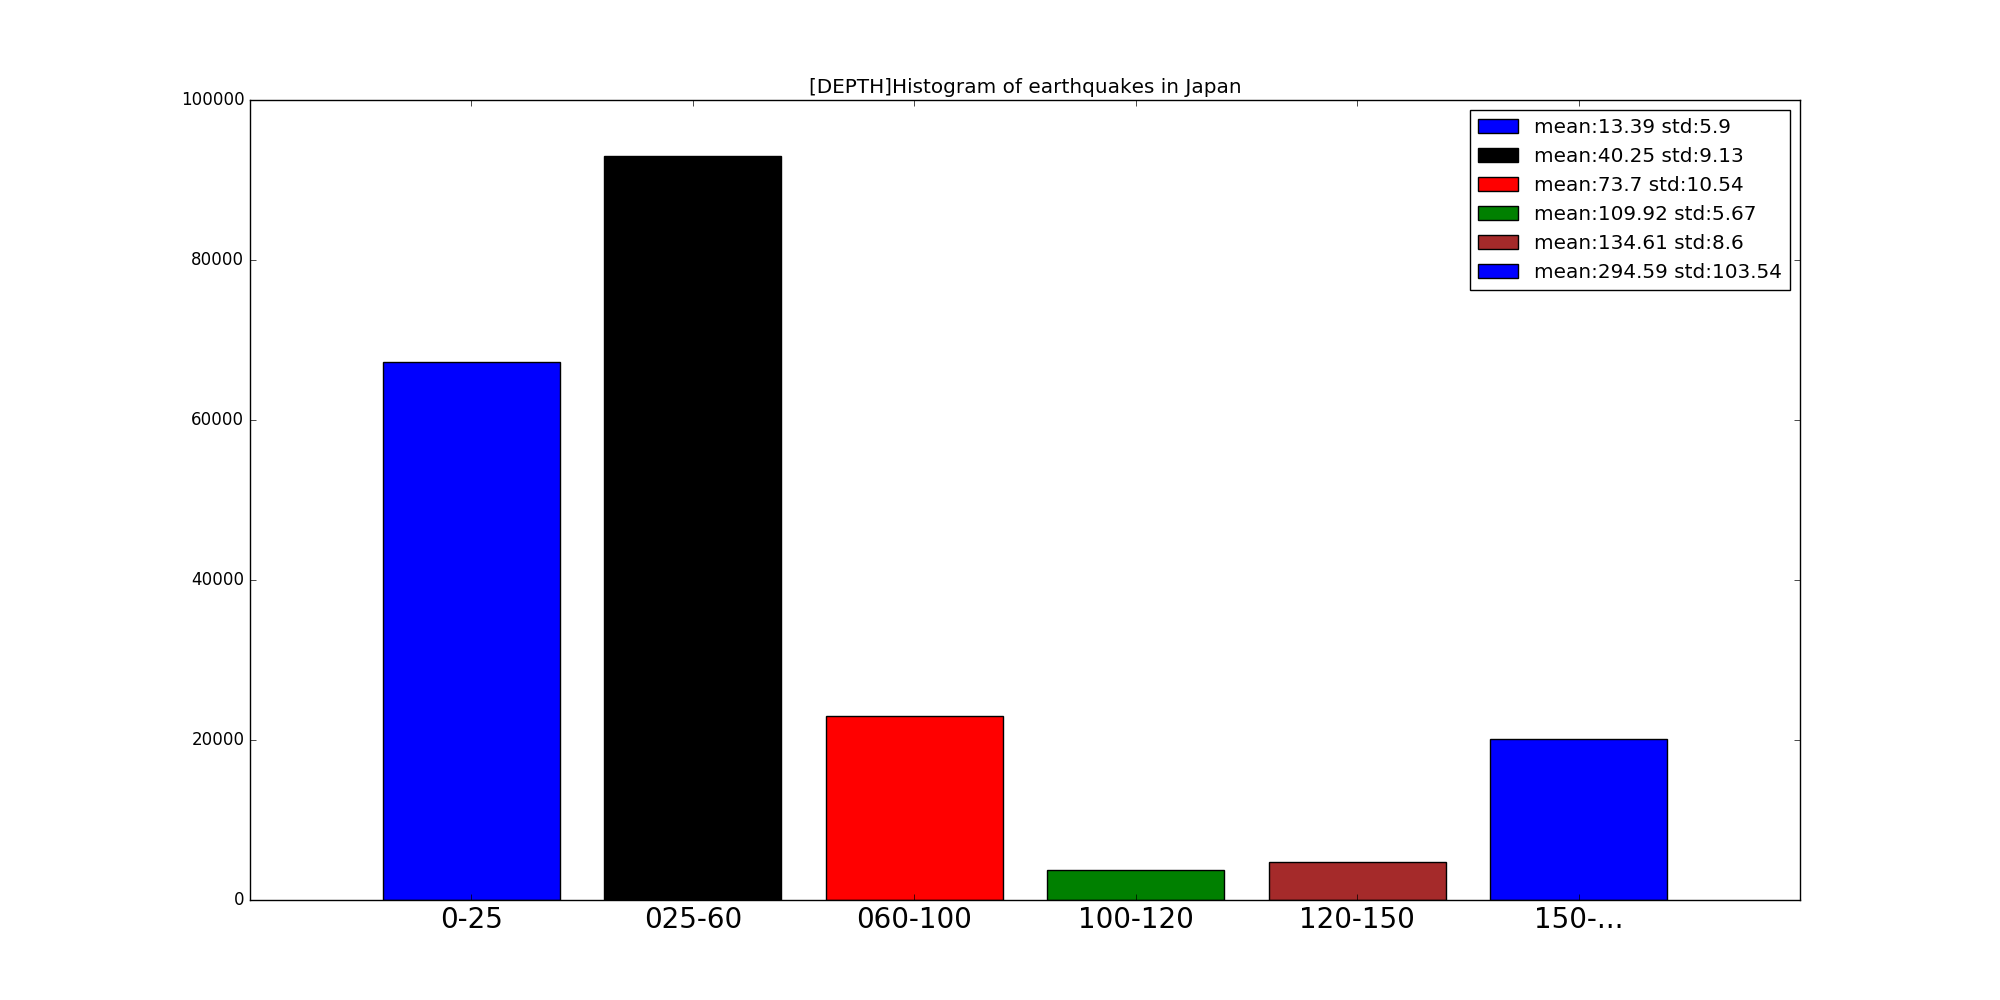
\includegraphics[scale=0.15]{img/detphsNew.png}
	\caption{Depth Histogram of earthquakes.}
	\label{histogramQuakes}
\end{figure}

The reason we decided to groups as: earthquakes with depth until 25
km, until 60 km or until 100 km. This is because shallow earthquakes
are considered to be more independent
earthquakes~\cite{yamanaka1990scaling}.

\begin{figure}
	\centering
	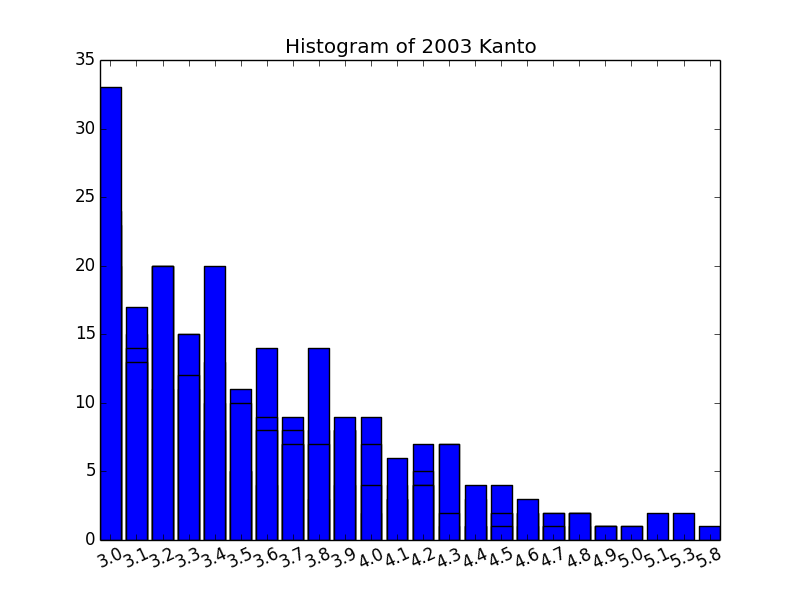
\includegraphics[scale=0.35]{img/Magnitude2003Kanto.png}
	\caption{Histogram of earthquakes stronger than 3.0 in Kanto}
	\label{quakesKanto}
\end{figure}
